%!TEX root = ../thesis.tex
%*******************************************************************************
%*********************************** First Chapter *****************************
%*******************************************************************************

\chapter{The Theory of Neutrino Physics}\label{chap:theory}
\setlength{\epigraphwidth}{.45\textwidth}
\epigraph{\textit{Light\\Light\\The visible reminder of Invisible Light}}{\textit{The Rock}\\\textsc{T. S. Eliot}}
\setlength{\epigraphwidth}{.4\textwidth}

\section{The Standard Model and Neutrinos}
% \subsection{A Brief Introduction to the Standard Model}
% Covering how the SM works at the highest level, including:
% \begin{itemize}
%     \item Quantum Field Theory and the Lagrangian dynamical framework
%     \item The connection between symmetries of a QFT model and its gauge fields that describe the model's forces
%     \item The SM's fundamental symmetries, and associated forces, but ---
%     \item Not (exactly) what we see ``normally''! The electromagnetic and weak forces appear distinct, and the weak gauge bosons have mass. To explain this, we need a further component, the Brout-Englert-Higgs (BEH) Mechanism. 
% \end{itemize}
% [2 pages total]
% \subsection{Neutrinos within the Standard Model}
\nomenclature{\textbf{SM}}{The Standard Model of Particle Physics}
The \textit{Standard Model} (SM) of Particle Physics is the culmination of a century's work by scientists to understand the fundamental constituent elements of the Universe, and their interactions. Within the SM, fundamental particles are excitations of associated quantum fields within spacetime. The particles that define the SM are shown in Fig.~\ref{fig:sm_particles}. As can be seen, these particles can be split into categories based on their properties.

\begin{figure}
    \centering
    % \includegraphics[]{}
    \caption[]{}
    \label{fig:sm_particles}
\end{figure}

One class of particles in the SM are known as the neutrinos, $\nu$: these are spin-$1/2$ fermions which are neutral in both the strong and electromagnetic force. The only means by which they are known to interact is through the weak nuclear force. There are three `flavours' of neutrino, one associated with their charged lepton counterparts: the electron neutrino $\nu_e$, the muon neutrino $\nu_\mu$, and the tau neutrino $\nu_\tau$.

\nomenclature{\textbf{EW}}{Electroweak (Theory)}
Crucial to understanding the nature of neutrinos is their interactions with other particles. Within the SM, the weak nuclear force and electromagnetism are unified into the Electroweak (EW) Theory by the work of Glashow, Salam, and Weinberg~\cite{}. % Cite foundational EW papers
This is a so-called \textit{chiral gauge field theory}. A quantum field theory is defined in terms of a Lagrangian density $\mathcal{L}$, from which one can determine the equations of motion of the fields and their associated particles. Gauge field theories are a special type of field theory which demand that the Lagrangian be invariant under certain kinds of transformation, beyond the basic requirement that the theory satisfies the requirements of special relativity. For EW, the Lagrangian is invariant under `local' transformations of the fields' internal degrees of freedom, defined by the `gauge' group $SU(2)_{L}\times U(1)_{Y}$, where $L$ and $Y$ are known as the left-handed weak and weak hypercharge, respectively.

A local transformation is one which changes values of the fields at all points in spacetime. By demanding invariance under these gauge transformations, as well as Lorentz invariance, the theory naturally predicts the existence of vector (spin-1) boson particles. These are known as the `gauge' bosons of the theory, and they mediate the interactions defined by the gauge group. The massive $W^{\pm}$ and $Z$ bosons, discovered by XXXXX in XXXX~\cite{}, % CITE!!!
mediate the weak nuclear force, whilst the massless photon $\gamma$ mediates the electromagnetic force.

The theory of EW interactions is also \textit{chiral}. Any spinor that defines the wavefunction of a spin-$1/2$ field can be split into its left- and right-handed `chiral' components, defined through the projection operators $P_{L,R} = \frac{1\mp\gamma^{5}}{2}$. The force associated with the $SU(2)_{L}$ part of the EW gauge group only interacts with the left-handed components of particles, denoted with the subscript $L$ on their wavefunction.

\nomenclature{\textbf{NC}}{Neutral Current (weak interaction)}
\nomenclature{\textbf{CC}}{Charged Current (weak interaction)}
The Lagrangian that defines the weak interactions of neutrinos is:
\begin{equation}
    -\mathcal{L} = \frac{g}{2\cos{\theta_{W}}}\sum_{\ell,L}\bar{\nu}_{\ell,L}\gamma^{\mu}\nu_{\ell,L}Z^{0}_{\mu}
    +\frac{g}{\sqrt{2}}\sum_{\ell}\bar{\nu}_{\ell,L}\gamma^{\mu}\ell^{-}_{L}W^{+}_{\mu} + \mathrm{h.c.}.
\end{equation}
Here, $g$ is the dimensionless coupling constant associated with $SU(2)_{L}$, and $\theta_{W}$ is the Weinberg angle. The three lepton flavour fields are denoted by $\ell=e,\mu,\tau$, with their associated neutrino fields being given by $\nu_{\ell}$. Similarly, the fields associated with the weak gauge bosons are given by $W^{\pm}$ and $Z^{0}$. The two components of this Lagrangian are known as the Neutral Current (NC) and Charged Current (CC) weak interactions of neutrinos, respectively. Similar Lagrangians exist that define the NC and CC interactions of quarks, as well as the NC interactions of the charged leptons.

\nomenclature{\textbf{IBD}}{Inverse $\beta$-decay}
Solidifying this theoretical picture are decades-worth of experimental tests of neutrinos and their place in the SM. The first neutrinos to be detected were electron anti-neutrinos, by Cowan and Reines in 1956~\cite{cowanDetectionFreeNeutrino1956,reinesNeutrino1956}. % cite Reines and Cowen.
These neutrinos were generated in the $\beta$-decay of radioactive isotopes within the Savannah River nuclear reactor: \ce{n \to p + e^{-} + \bar{\nu}_{e}}. This decay arises from a down quark within the neutron of an atom converting into an up quark via a CC interaction, generating a virtual $W^{-}$ boson that promptly decays into an electron and $\bar{\nu}_{e}$. The method by which Cowen and Reines detected these anti-neutrinos was through \textit{inverse $\beta$-decay} (IBD): \ce{\bar{\nu}_{e} + p \to e^{+} + n}. This process also originates from CC interactions. Analogous CC interactions allowed Danby \textit{et al} to discover the muon neutrino in 1962~\cite{danbyObservationHighEnergyNeutrino1962}, % cite Lederman, Schwarts, Steinberger
and the DONUT Collaboration to discover the tau neutrino in 2000~\cite{kodamaObservationTauNeutrino2001}. % cite DONUT Collaboration

The existence of NC interactions with neutrinos and anti-neutrinos was first demonstrated by the Gargamelle experiment in 1974~\cite{hasertObservationNeutrinolikeInteractions1973,hasertSearchElasticMuonneutrino1973,hasertObservationNeutrinolikeInteractions1974,blietschauEvidenceLeptonicNeutral1976}. % cite gargamelle
In particular, the observation of anti-muon neutrino electron elastic scattering, \ce{\bar{\nu}_{\mu} + e^{-} \to \bar{\nu}_{\mu} + e^{-}} by the experiment was an unambiguous demonstration of NC interactions. Further experiments, such as CHARM2, demonstrated the consistency of observed NC interactions with EW theory~\cite{}. % cite CHARM2 relevant paper(s)

In 1958, Goldhaber \textit{et al}~\cite{goldhaberHelicityNeutrinos1958} were able to demonstrate experimentally that the helicity of electron neutrinos, i.e. the component of their spin along the direction of motion, is $-1$. No evidence of neutrinos with positive helicities (or equally, anti-neutrinos with negative helicities) exists. This stands in firm contrast to all other SM particles.

No flavours of neutrino beyond the electron, muon, or tau types have been discovered. A combined analysis of data from the four LEP experiments looking at the decay width of the $Z$ boson was able to indirectly measure the number of neutrino species that could undergo NC interactions and had masses less than one half of the $Z$ boson: $N_{\nu} = 2.9963\pm0.0074$~\cite{}. % cite LEP papers, including update with correction!
This measurement is very strong evidence that no other `light' neutrinos exist.


% \begin{itemize}
%     \item Basic description of where neutrinos fit into SM: 3 kinds of neutral fermion, the counterparts to the charged fermions. Interacts with the weak force only.
%     \item Summary of the experimental evidence for this picture: mainly, the discovery of electron anti-neutrinos by Cowan and Reines, the muon neutrino by Lederman, Schwartz, and Steinberger, and the tau neutrino by the DONUT Collaboration. Further critical experiments include the first measurement of a neutrino's helicity by Goldhaber et al. as well as Danby et al.'s demonstration that $\nu_{\mu}$ are distinct from $\nu_{e}$.
%     \item More detailed description, via Feynman diagrams, of the two fundamental modes of interaction by neutrinos with the weak force: charged- and neutral-current interactions. A brief mention of the quantitative theory that underlies description: Gashow, Salam, and Weinberg's Electroweak Theory. This explains not only the V--A structure of charged-current interactions, but also predicted accurately the nature of neutral-current interactions. (Given space constraints, I see no reason to go into much of the details of the theory, or the many experimental tests of its structure.)
% \end{itemize}

% [4 pages]
\section{Neutrino Oscillations and Neutrino Masses}
So far in this description, no attempt has been made to explain the origin of the masses of the fundamental particles. It is certainly straightforward to na\"{i}vely add a mass term such as $m_{e}\bar{e}_{L}e_{R}$ into the SM Lagrangian, where $m_e$ is the mass of the electron. However, one can show that any mass terms added will necessarily violate the $SU(2)_{L}\times U(1)_{Y}$ symmetry that defines the EW interactions~\cite{}. % should cite something appropriate.
The weak vector bosons $W^{\pm}$ and $Z$ would then need to be massless, in contradiction with observations.

\nomenclature{\textbf{BEH}}{Brout-Englert-Higgs (Mechanism)}
The solution to this problem comes in the form of the \textit{Brout-Englert-Higgs (BEH) Mechanism}~\cite{}, % cite BEH theory papers
the final component of the SM.  In this Mechanism, an additional two-component ``Higgs'' field $H$ is proposed, which is able to interact with the other fields of the theory in a manner that preserves the SM gauge symmetries. One such part of the added Higgs field interactions are the so-called Yukawa terms~\cite{}, % cite Yukawa, presumably
which for interactions with leptons are given by:
\begin{equation}
    -\mathcal{L}_{\mathrm{Yukawa,lep}} = \sum_{\ell}y_{\ell}\bar{L}^{\ell}H\ell^{c} + \mathrm{h.c.},
\end{equation}
where $y_{\ell}$ are the ``Yukawa'' coupling constants for the three lepton flavours, $L^{\ell} = \begin{pmatrix}
    \nu_{\ell,L} \\ \ell_{L}
\end{pmatrix}$ are the left-handed lepton doublets of the SM, and $\ell^{c}$ are the right-handed charged leptons.

The key to the BEH Mechanism is \textit{Spontaneous Symmetry Breaking}: the Higgs field is defined in such a way that the ground state takes a non-zero `vacuum expectation value', $v$. By doing so, the underlying gauge symmetry of the EW interactions is spontaneously broken as $SU(2)_{L}\times~U(1)_{Y}\to~U(1)_{Q}$, where $U(1)_{Q}$ is the residual electromagnetic charge conservation. The above Yukawa Lagrangian term after symmetry breaking generates the mass terms for the charged leptons:
\begin{equation}
    -\mathcal{L}_{\mathrm{Yukawa,lep}} \to \sum_{\ell}m_{\ell}\bar{\ell}_{L}\ell^{c} + \mathrm{h.c.},
\end{equation}
where $m_{\ell} = \frac{v}{\sqrt{2}}y_{\ell}$ are the charged lepton masses. Other terms associated with Higgs interactions in the SM generate mass terms for the quarks and weak vector bosons, as seen in data. A further prediction of this BEH Mechanism is the existence of a massive scalar boson known as the Higgs particle; this was discovered in 2012 by the ATLAS and CMS Collaborations~\cite{}. %cite Higgs discovery papers

The one type of fundamental particle not covered by the above argument are neutrinos. If neutrinos were massless, then there is no issue: we observe neutrinos to have only negative helicities, which is equal to left-handed chiralities if they are massless. As the SM contains no right-handed neutrinos, no Yukawa interaction can be built to generate masses for the neutrinos. One can also demonstrate that, in the SM, neutrinos cannot even obtain masses through loop corrections~\cite{}. % cite PDG review 14

This assumption of massless neutrinos appears initially consistent with the current observations of direct neutrino mass measurements. The strongest direct limits come from the KATRIN experiment, which looks at the endpoint of the tritium $\beta$-decay spectrum. The `effective'\footnote{
    KATRIN measures the `effective' mass and not the actual mass, because of the phenomenon of neutrino oscillations as described in the following sections.
} electron anti-neutrino mass $m_{\nu} < \SI{0.8}{\eV}$ at a 90\% confidence level~\cite{}. % cite https://inspirehep.net/literature/1863711
Even stronger limits are available from cosmology, by looking in part at the power spectrum of the Cosmic Microwave Background. Assuming the so-called Standard `$\Lambda$CDM' Model of Cosmology, limits on the sum of all three neutrino flavours $\sum m_{\nu}<\mathcal{O}(\SI{0.1}{\eV})$ have been achieved~\cite{}. % cite a couple of papers, maybe.

\subsection{The Evidence for Neutrino Oscillations}\label{sec:nu_osc_evidence}
Despite the current lack of any direct measurements, we now know that at least some neutrinos must have mass. This is because of the phenomenon of \textit{neutrino oscillations}, which have been observed over a variety of experiments and contexts. The critical pieces of evidence for this process are described here; the underlying mathematical model that is used to explain them quantitatively is described in Section~\ref{sec:nu_osc_phenom}.

\subsubsection{The Solar Neutrino Problem}
\nomenclature{\textbf{SSM}}{Standard Solar Model}
Neutrinos are generated from the Sun as a by-product of the fusion reactions at its core. At the highest level, protons fuse into alpha particles by the overall reaction \ce{4p \to ^{4}He{} + 2e^{+} + 2\nu_{e}}, generating also $\sim\SI{25}{\MeV}$ of energy that enables the Sun to shine~\cite{}. % cite Bahcall Neutrino Astrophysics.
This process is known as `hydrogen burning'. The Standard Solar Model (SSM) is the current best quantitative description of stellar evolution for main sequence stars, and our Sun in particular. It covers the nuclear reactions that generate both the energy that powers the star and the changes in the relative isotopic abundances, how the energy is transported out through the star via radiation of photons and convection, and how the outward pressures caused by this radiation is balanced by gravity to maintain hydrostatic equilibrium. An introduction to the SSM can be found in~\cite{}. % cite Bahcall's book again.

In the Sun, two sets of nuclear reactions enable hydrogen burning to occur: the \textit{proton-proton (pp) chain} and \textit{CNO cycle}. Diagrams of these reaction chains are shown in Fig.~\ref{fig:pp_chain} and Fig.~\ref{fig:cno_cycle}, respectively. In the pp chain, protons are first fused together to form a \ce{^{2}H} nucleus through the `pp' and `pep' reactions, the latter also using an electron. Both of these processes are weak interactions that generate an electron neutrino. Once a deuterium nucleus has been generated, it strongly interacts with a proton to create a \ce{^{3}He} nucleus. The dominant method for hydrogen burning to then terminate is for two \ce{^{3}He} nuclei strongly interact to generate \ce{^{4}He} and two protons.

\begin{figure}
    \centering
    % \includegraphics[]{}
    \caption[]{}
    \label{fig:pp_chain}
\end{figure}

\begin{figure}
    \centering
    % \includegraphics[]{}
    \caption[]{}
    \label{fig:cno_cycle}
\end{figure}

Two other nuclear reactions with \ce{^{3}He} are possible. In one, \ce{^{3}He} fuses with \ce{^{4}He} to generate a \ce{^{7}Be} nucleus, which can then generate a neutrino either from the creation of \ce{^{7}Li} via electron capture, or from the additional fusing into \beight{} which promptly $\beta^{+}$-decays. These are known as the \ce{^{7}Be} and \beight{} solar neutrino generation reactions, respectively. The final and rarest reaction within the pp chain that generates a neutrino is the so-called `hep' reaction, in which \ce{^{3}He} directly fuses with a proton.

The CNO cycle is a secondary means by which the Sun can burn hydrogen. This is achieved through the aid of a \ce{^{12}C} nucleus as a catalyst. Part of the cycle involves the generation of unstable isotopes \ce{^{13}N} and \ce{^{15}O}, both of which \ce{\beta^{+}}-decay, creating electron neutrinos. In a rare side-chain of the CNO cycle, it is possible to also generate \ce{^{17}F} which also weakly decays to generate a neutrino. This is the final method of generating neutrinos in our Sun.

The SSM quantitatively predicts the flux and energy spectra of neutrinos generated through each of the above processes, as incident on the Earth. This is shown in Fig.~\ref{fig:ssm_neutrino_spectra}. The shapes of the energy spectra are determined by the nuclear reactions that define the process: for example, the broad shape of the \beight{} $\nu_{e}$ energy spectrum comes from the $\beta^{+}$-decay of \beight{} isotopes, and has been measured in nuclear beam experiments to high precision~\cite{winterB8NeutrinoSpectrum2006}. % citation of B8 shape measurement by Winter et al.

\begin{figure}
    \centering
    % \includegraphics[]{}
    \caption[]{}
    \label{fig:ssm_neutrino_spectra}
\end{figure}

The rate of the \beight{} interaction in the Sun, and hence the generated neutrino flux, depend strongly on the radial temperature distribution of the Sun, the cross-sections of the pp chain nuclear reactions, and the Sun's chemical composition. The latter point remains a topic of some controversy: measurements of the relative abundances in 1998 through spectroscopy of the Sun's photosphere as well as meteorites give a `metal-to-hydrogen' ratio of $Z/X = 0.023$~\cite{grevesseStandardSolarComposition1998}, whereas a more recent study in 2009 has a substantially lower value of $Z/X = 0.018$~\cite{asplundChemicalCompositionSun2009}. Metallicity here is used in the astrophysical sense: elements heavier than hydrogen or helium. These two models are called the `high-metallicity' \texttt{GS98} model and `low-metallicity' \texttt{AGSS09met} model, respectively. The current best SSM associated with these two abundance models, denoted \texttt{B16\_GS98} and \texttt{B16\_AGSS09met}, have \beight{} flux predictions of $\Phi_{\beight{}} = (5.46\pm12\%)\times 10^{6}\,\si{\per\cm\squared\per\second}$ and $\Phi_{\beight{}} = (4.50\pm12\%)\times 10^{6}\,\si{\per\cm\squared\per\second}$, respectively~\cite{vinyolesB16StandardSolar2018}.

\nomenclature{\textbf{SNU}}{Solar Neutrino Unit, defined as $10^{-36}$ neutrino interactions per second}
The first experiment built to measure solar neutrinos was that of the Homestake Chlorine Detector, starting in the late 1960s~\cite{davisSearchNeutrinosSun1968}. A large tank of \ce{C_{2}Cl_{4}} was put deep underground, whereby electron neutrinos could be captured by the \ce{^{37}Cl} nuclei: \ce{^{37}Cl{} + \nu_{e} \to ^{37}Ar{} + e^{-}}. Through a careful chemical extraction process, any atoms of \ce{^{37}Ar} generated in the tank could be counted with an efficiency over 90\%. After running the experiment for a period of almost 30 years, a final measurement of the solar neutrino interaction rate was $2.56\pm0.16(\mathrm{stat.})\pm0.16(\mathrm{sys.})\mathrm{ SNU}$~\cite{clevelandMeasurementSolarElectron1998}, % cite Ray davis
where 1 SNU (`Solar Neutrino Unit') is defined as $10^{-36}$ events per target atom per second. The results as a function of time can be seen in Fig.~\ref{fig:homestake_results}.

\begin{figure}
    \centering
    % \includegraphics[]{}
    \caption[]{}
    \label{fig:homestake_results}
\end{figure}

In contrast, according to one particular recent SSM using the GS98 metallicity model, the expected rate is $84.6^{+0.87}_{-0.88}\mathrm{ SNU}$~\cite{pena-garaySolarNeutrinosSolar2008}, highly inconsistent with the results at Homestake. This disagreement became known as the \textit{Solar Neutrino Problem}, and was the first piece of evidence towards neutrino oscillations.

Since the Homestake experiment, a series of solar neutrino experiments used a variety of different target isotopes to measure the rate of solar neutrinos. In all cases, the measured rates were substantially below what is expected from the SSM. The SAGE and GALLEX/GNO experiments used the capture of electron neutrinos on \ce{^{71}Ga} to measure the capture rate: the final observations were $65.4^{+3.1}_{-3.0}(\mathrm{stat.})\,^{+2.6}_{-2.8}(\mathrm{sys.})\,\mathrm{ SNU}$~\cite{abdurashitovMeasurementSolarNeutrino2009} and $69.3\pm4.1\pm3.6\,\mathrm{ SNU}$~\cite{altmannCompleteResultsFive2005}, respectively. An SSM expectation is $127.9^{+8.1}_{-8.2}$~\cite{pena-garaySolarNeutrinosSolar2008}. Because the capture on \ce{^{71}Ga} has a much lower energy threshold than \ce{^{37}Cl}, these experiments were able to show that the Solar Neutrino Problem was associated with the low-energy pp neutrinos as much as the higher energy \beight{} and \ce{^{7}Be} neutrinos.

\nomenclature{\textbf{ES}}{Elastic Scattering}
The Kamiokande experiment, and its successor Super-Kamiokande, are large water Cherenkov detectors, sensitive to neutrinos through neutrino-electron elastic scattering (ES): $\nu_{x} + e^{-}\to\nu_{x} + e^{-}$. All flavours of neutrino are capable of scattering through a NC process, but there is an additional CC mode for electron neutrinos, as shown in Fig.~\ref{fig:nu_e_es_feynman_diagrams}. The differential cross-section for this interaction as a function of the scattered electron's kinetic energy $T$ is given by~\cite{bahcallSolarNeutrinosRadiative1995}: % cite Bahcall
\begin{align}\label{eq:enu_es_xsec}
    \frac{d\sigma_{\nu_{i}}}{dT} &= \frac{2G_{F}^{2}m_{e}}{\pi}\left\{
        g_{L}^{2}(T)\left[
            1 + \frac{\alpha}{\pi}f_{-}(z)
        \right]
        + g_{R}^{2}(T)(1-z)^{2}\left[
            1 + \frac{\alpha}{\pi}f_{+}(z)
        \right]\right.\nonumber\\
        &\qquad \left. {}
        -g_{R}(T)g_{L}(T)\frac{m_{e}}{E_{\nu}}\left[
            1 + \frac{\alpha}{\pi}f_{+-}(z)
        \right]
    \right\},
\end{align}
where $i = e, \mu$\footnote{
    $\frac{d\sigma_{\nu_{\mu}}}{dT} = \frac{d\sigma_{\nu_{\tau}}}{dT}$ because both flavours of neutrino only undergo the NC interaction.
}, $G_{F}$ is the Fermi coupling constant, $m_{e}$ is the electron mass, $\alpha$ is the fine-structure constant, $E_{\nu}$ is the incident neutrino energy, and $z = T/E_{\nu}$. $g_{L,R}(T)$ are the left- and right-handed running chiral couplings, which have a $T$-dependence because of next-to-leading order EW and QCD corrections. Similarly, $f_{-}(z)$, $f_{+}(z)$, and $f_{+-}(z)$ are all QED radiative corrections. Fig.~\ref{fig:nu_e_es_xsec} shows this differential cross-section for both $\nu_{e}$ and $\nu_{\mu}$ scattering. As can be seen, the cross-section for $\nu_{e}$ is $\sim 6$ times that of $\nu_{\mu}$, because of the additional CC interaction mode.

\begin{figure}
    \centering
    % \includegraphics[]{}
    \caption[]{}
    \label{fig:nu_e_es_feynman_diagrams}
\end{figure}

\begin{figure}
    \centering
    % \includegraphics[]{}
    \caption[]{}
    \label{fig:nu_e_es_xsec}
\end{figure}

The most recent combined measurement of the \beight{} solar neutrino flux in Super-Kamiokande is $(2.345\pm0.014(\mathrm{stat.})\pm0.036(\mathrm{sys.}))\times10^{6}\,\si{\per\cm\squared\per\second}$~\cite{abeSolarNeutrinoMeasurements2016}, roughly half the amount expected from the SSM~\cite{vinyolesB16StandardSolar2018}.

\nomenclature{\textbf{SNO}}{Sudbury Neutrino Observatory}
\nomenclature{\textbf{UPW}}{Ultra-pure water}
One of the most important experiments for demonstrating that neutrino oscillations are the solution to the Solar Neutrino Problem was the Sudbury Neutrino Observatory, SNO. A large spherical acrylic vessel \SI{2.2}{\km} underground was filled with \num{1000} tonnes of heavy water, \ce{D_{2}O}, from which Cherenkov light due to particle interactions could be detected~\cite{BOGER2000172}. Neutrinos were able to interact with the heavy water via three complementary modes: the CC process \ce{\nu_{e} + d \to e^{-} + 2p}, the NC process \ce{\nu_{x} + d \to \nu_{x} + p{} + n}, and the ES process described above.

Results of the measured fluxes of $\nu_{e}$ and $\nu_{\mu,\tau}$ solar neutrinos for the three detection modes in SNO, ES results from Super-Kamiokande, and comparison to the SSM are shown in Fig.~\ref{fig:sno_flux_results}. Because the NC interaction is insensitive to neutrino flavour, it is able to directly measure the total flux of \beight{} solar neutrinos, regardless of flavour. One can see that, from the results, the NC flux measurement is consistent with the SSM. In contrast, the CC mode is only sensitive to the $\nu_{e}$ flux, whilst the ES mode is sensitive to an admixture of the different neutrino flavours. The results of all measurements of solar neutrinos from both SNO and Super-Kamiokande lead to consistent values of the flux of \beight{} neutrinos for each flavour, consistent also with the SSM.

\begin{figure}
    \centering
    % \includegraphics[]{}
    \caption[]{}
    \label{fig:sno_flux_results}
\end{figure}

% ADD BOREXINO, KamLAND results???

\subsubsection{The Atmospheric Neutrino Anomaly}
Atmospheric neutrinos come from the decays of cosmic ray pions and muons in the Earth's atmosphere. One can show that the expected ratio of the flux of muon neutrinos to electron neutrinos generated in the atmosphere should be about 2~\cite{}. % cite something!
The IBM~\cite{}, % cite
Kamiokande~\cite{}, % cite
and Super-Kamiokande~\cite{} % cite
experiments were able to detect atmospheric neutrinos through CC interactions with electrons in the water, generating electron or muon tracks (depending on the neutrino flavour) that could be distinguished by the shape of their Cherenkov rings. In all cases, the observed ratio of $\nu_{\mu}$ to $\nu_{e}$ events was consistently below expectations. This was known as the Atmospheric Neutrino Anomaly.

Super-Kamiokande was able to gather enough statistics from atmospheric neutrino interactions to demonstrate that there was a clear dependence on the rate of muon neutrino interactions as a function of the event direction. In particular, the asymmetry $A$ between the number of upward-going muon neutrino events $U$, and downward-going events $D$, was measured in one dataset to be~\cite{}: % cite SK
\begin{equation*}
    A = \frac{U-D}{U+D} = -0.296 \pm 0.048(\mathrm{stat.}) \pm 0.01(\mathrm{sys.}),
\end{equation*}
a deviation from zero by over 6$\sigma$. In contrast, the asymmetry measured for atmospheric $\nu_{e}$ events was consistent with zero. Further analysis on the experiment looked at the rate of atmospheric $\nu_{\mu}$ events as a function of the ratio $L/E$, where $L$ is the estimated distance from production of the neutrino, and $E$ is the neutrino energy. The relative rate compared to expectations is shown in Fig.~\ref{fig:LE_plot_SK_atmos}. Taken together, these atmospheric neutrino results demonstrate that there is a disappearance of muon neutrinos which depends on the ratio $L/E$, whereas there is no similar effect for the electron neutrinos.

\begin{figure}
    \centering
    \begin{subfigure}{0.48\textwidth}
        \centering
        % 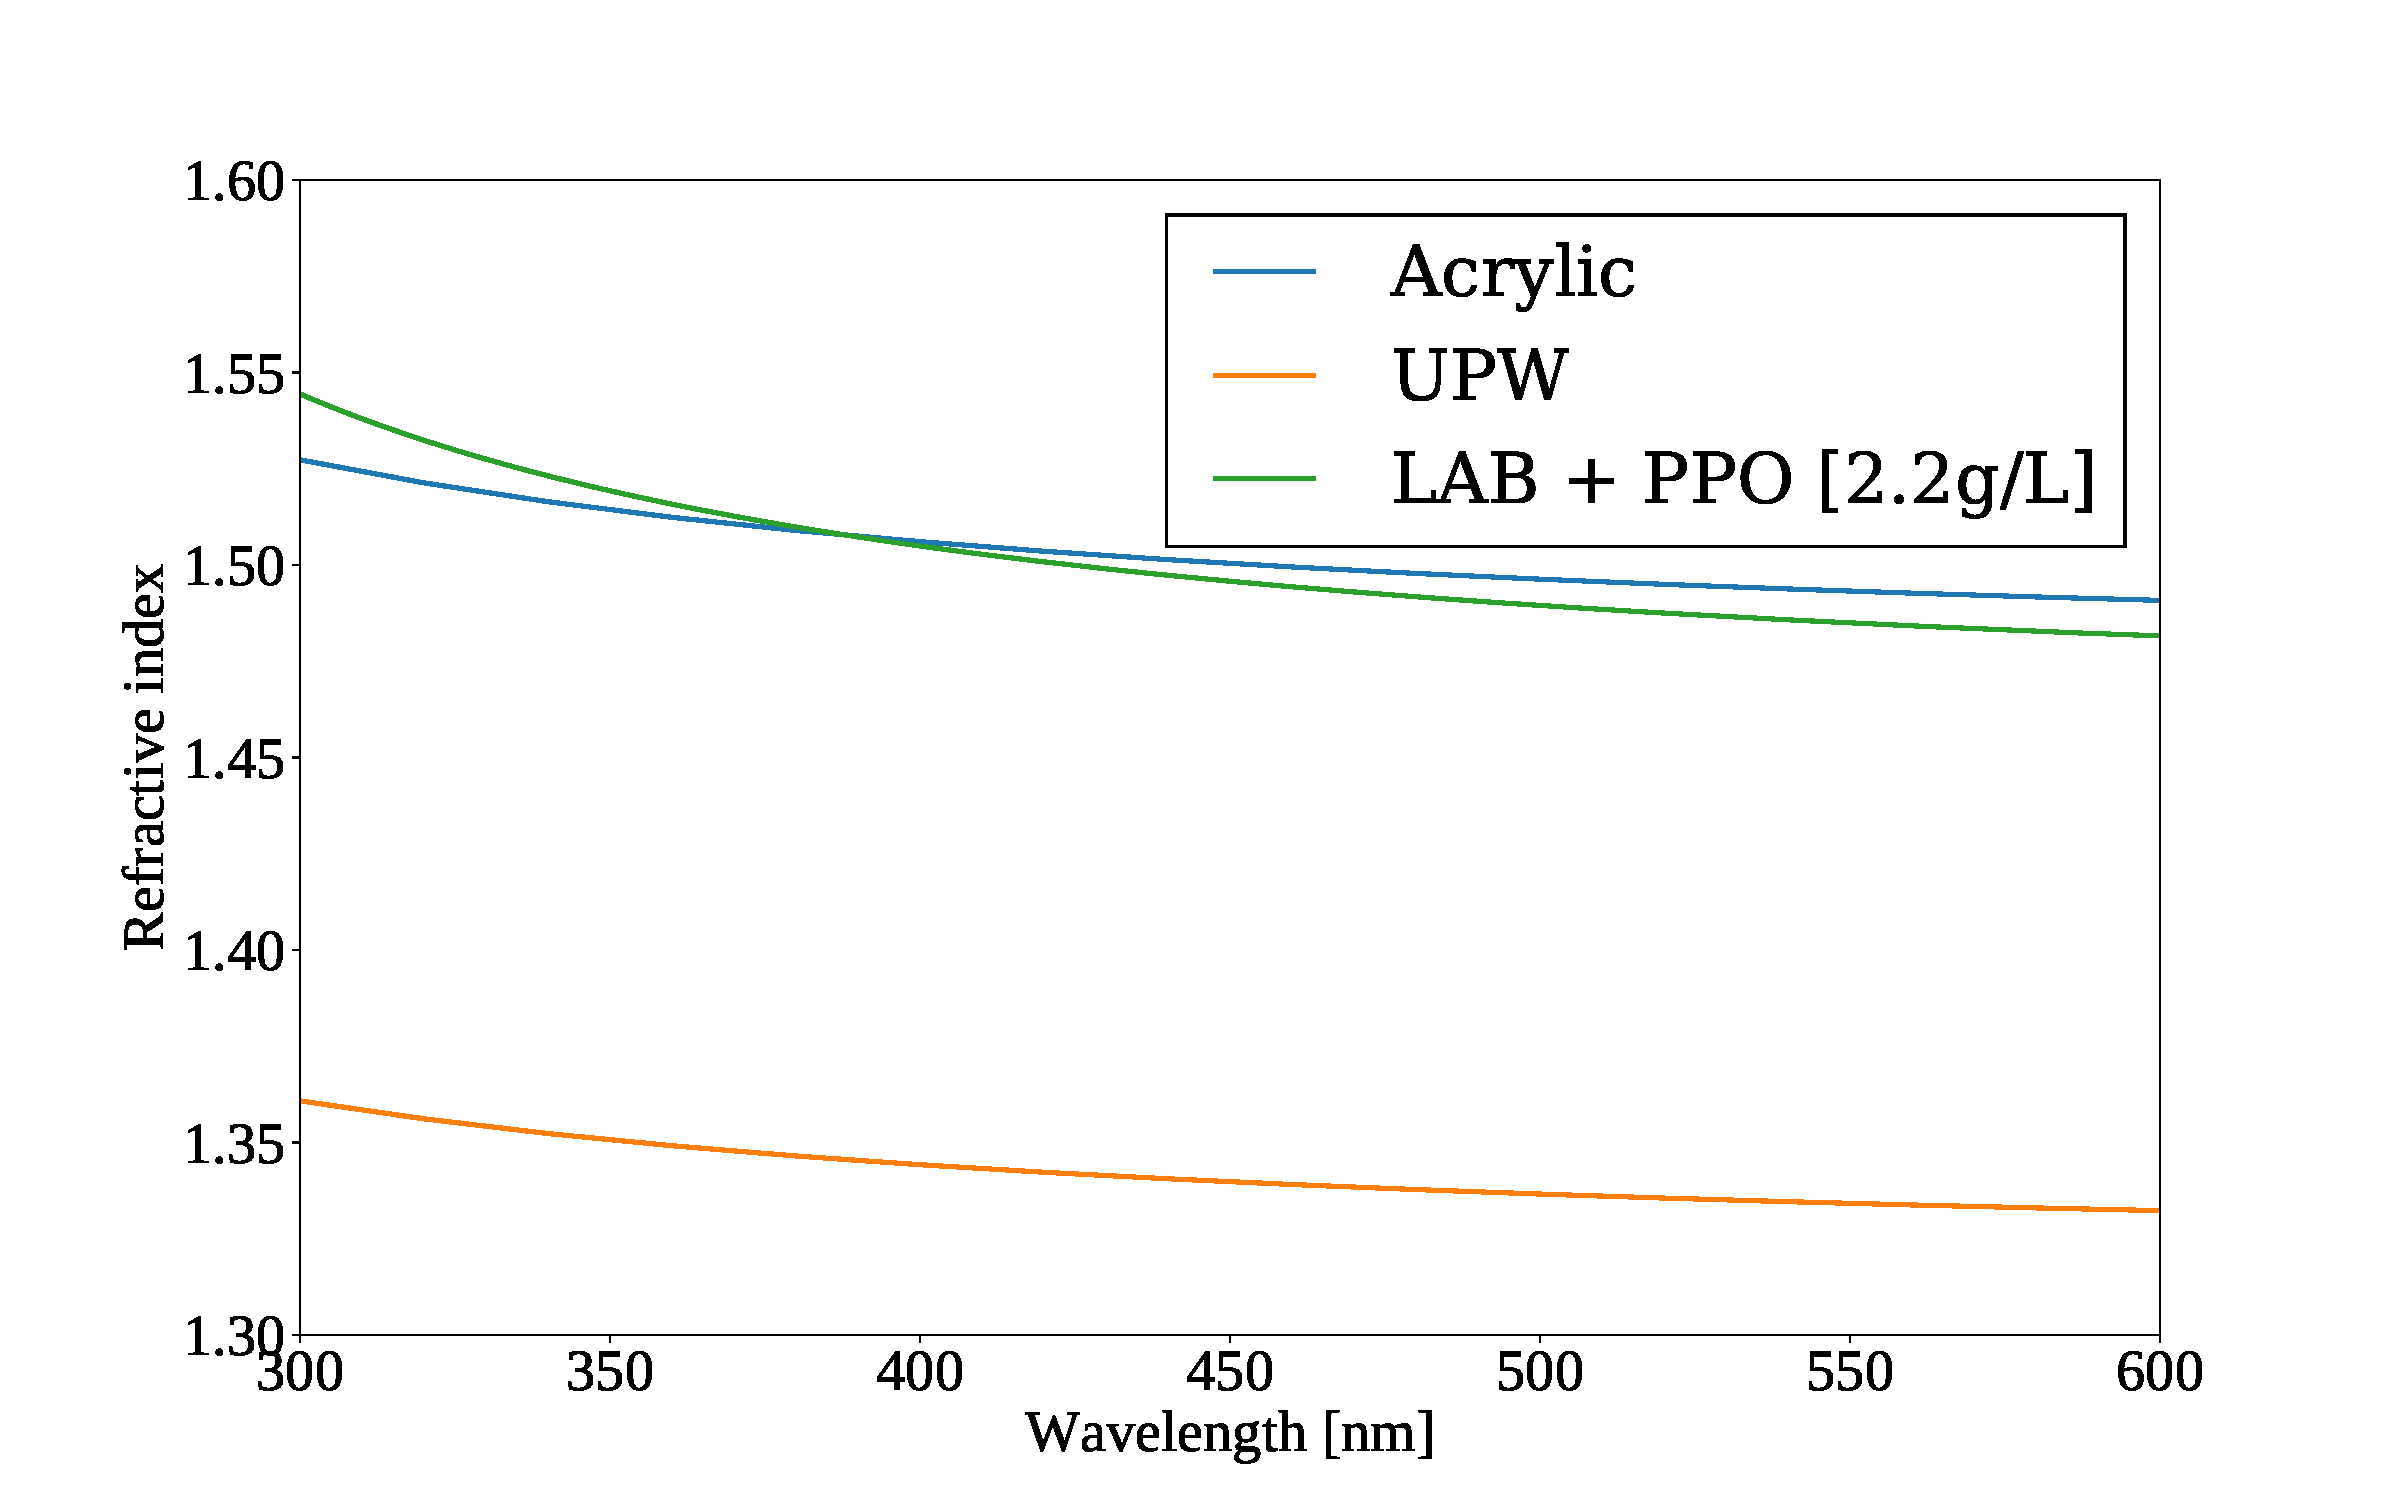
\includegraphics[width=0.95\linewidth]{2_Detector/Figs/refractive_indices_plot.pdf}
        \caption{}
        \label{fig:LE_plot_SK_atmos}
    \end{subfigure}
    \begin{subfigure}{0.48\textwidth}
        \centering
        % 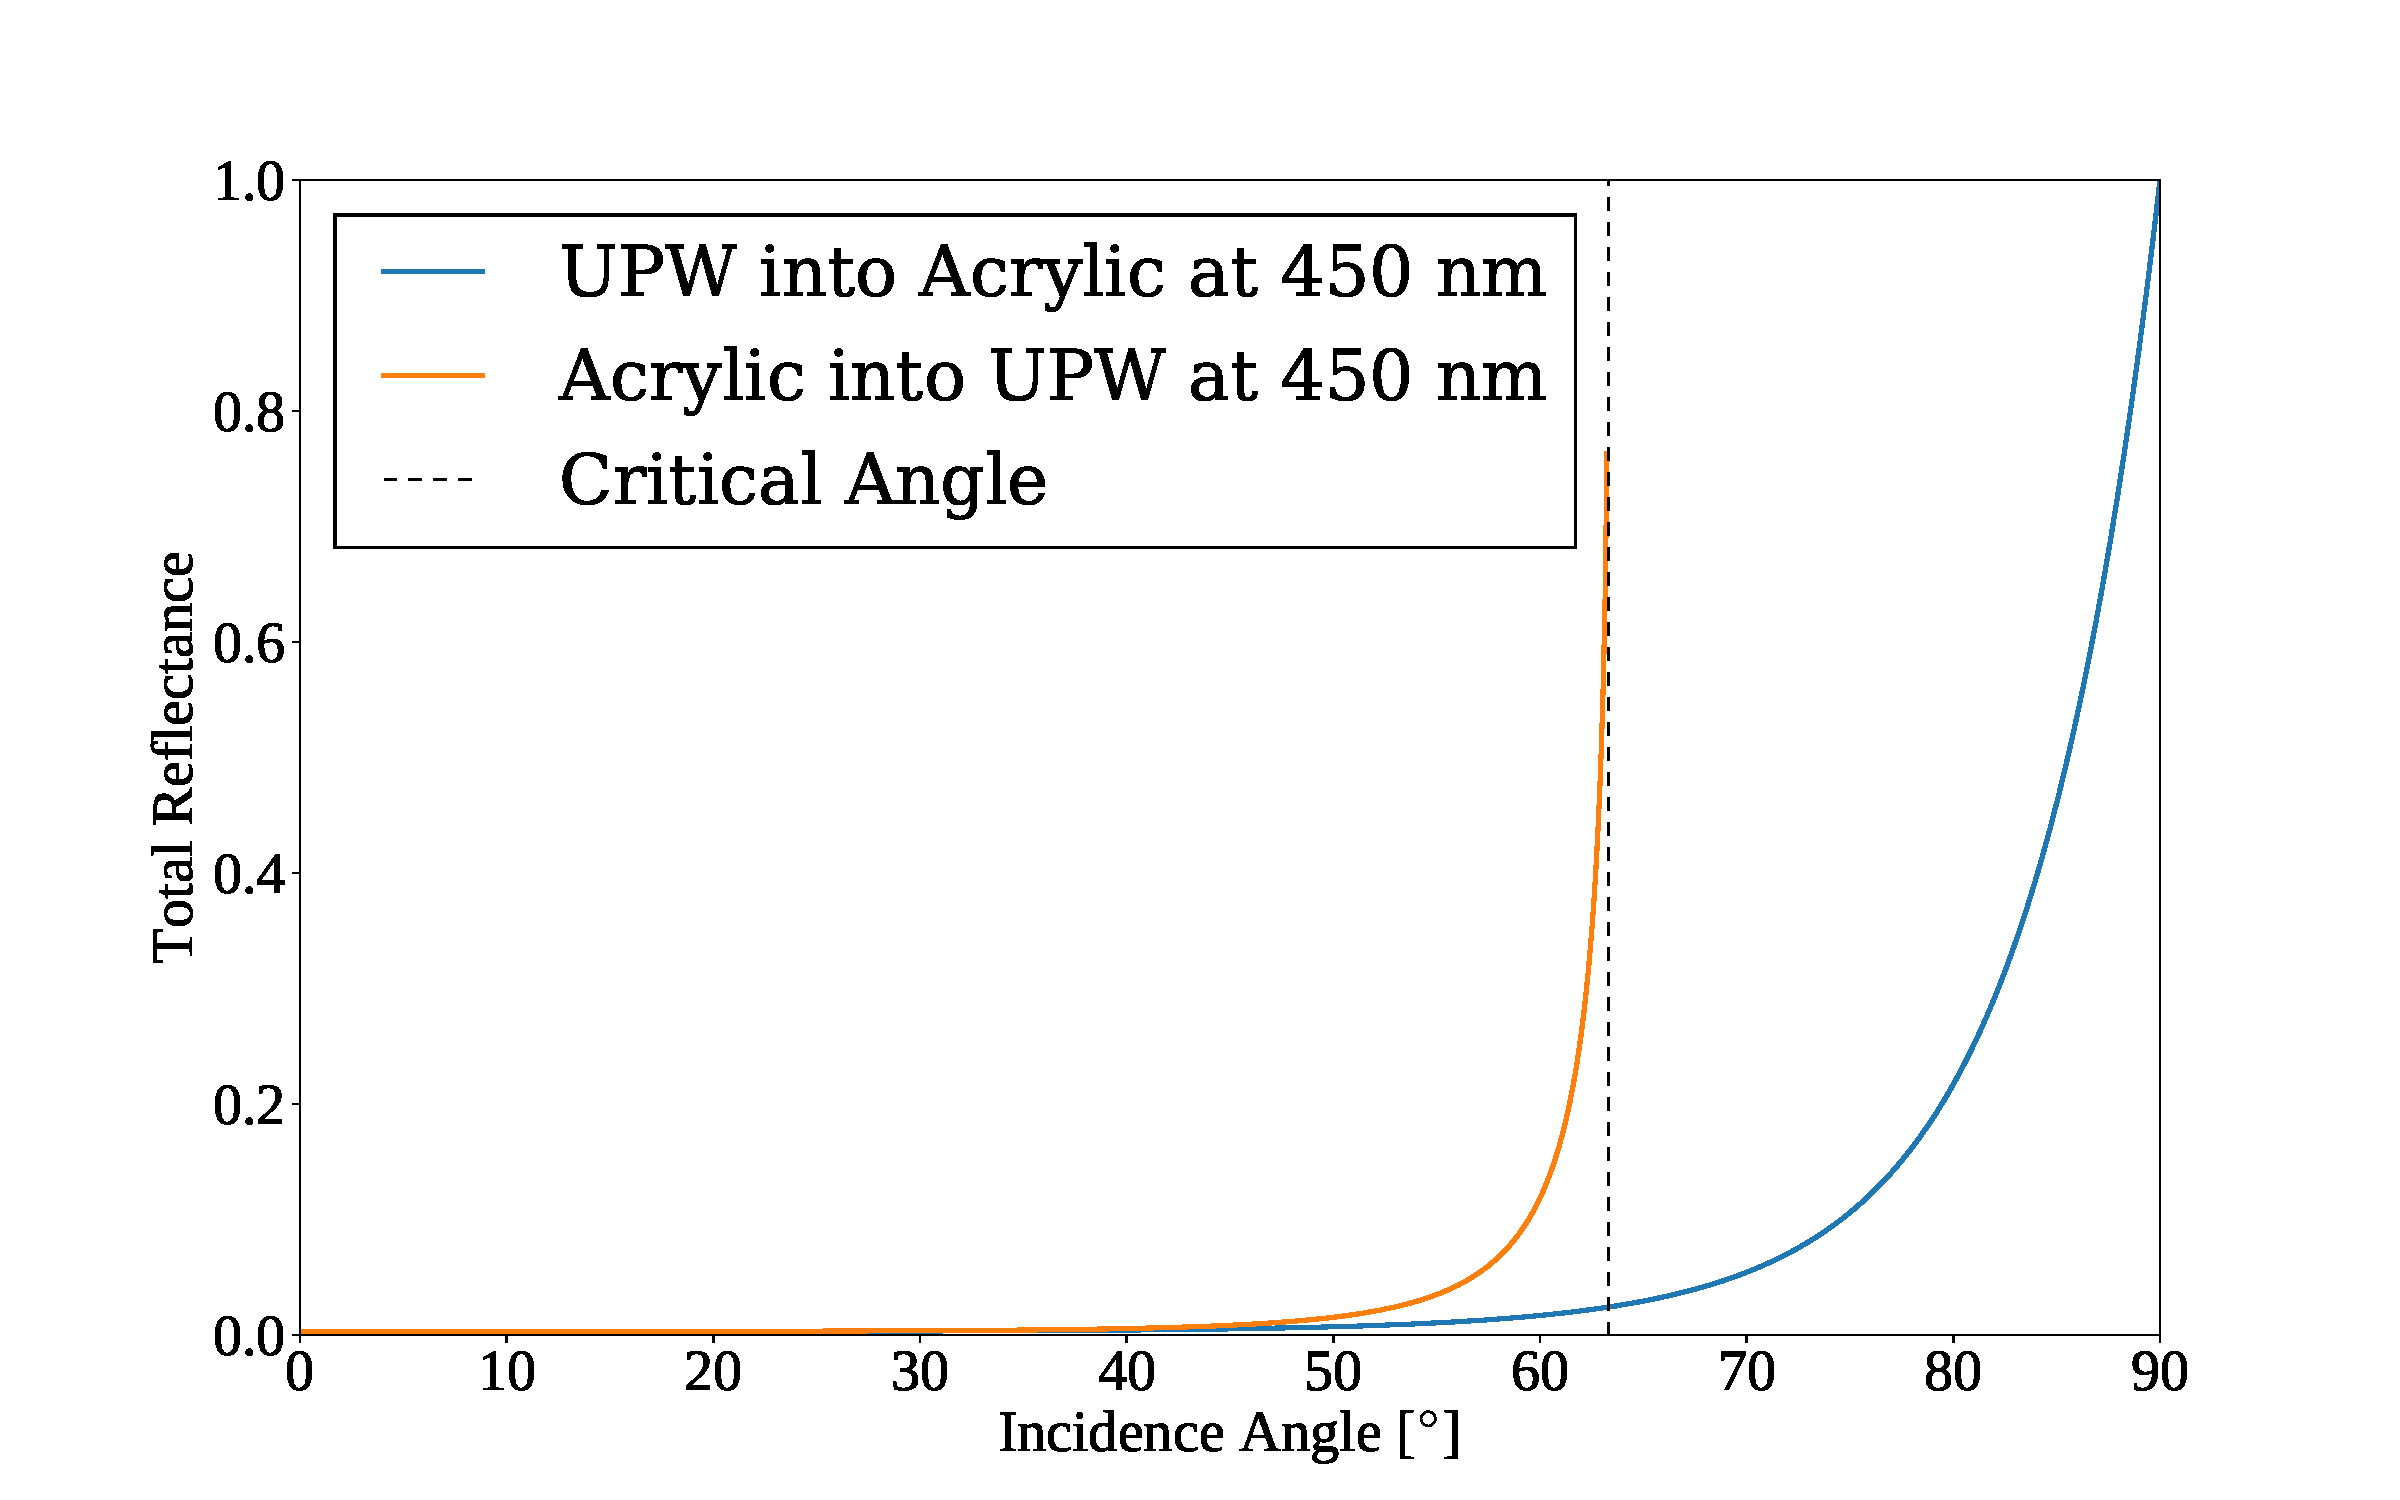
\includegraphics[width=0.95\linewidth]{2_Detector/Figs/reflectance_vs_angle_plot.pdf}
        \caption{}
        \label{fig:LE_plot_KamLAND_antinu}
    \end{subfigure}
    \begin{subfigure}{0.48\textwidth}
        \centering
        % 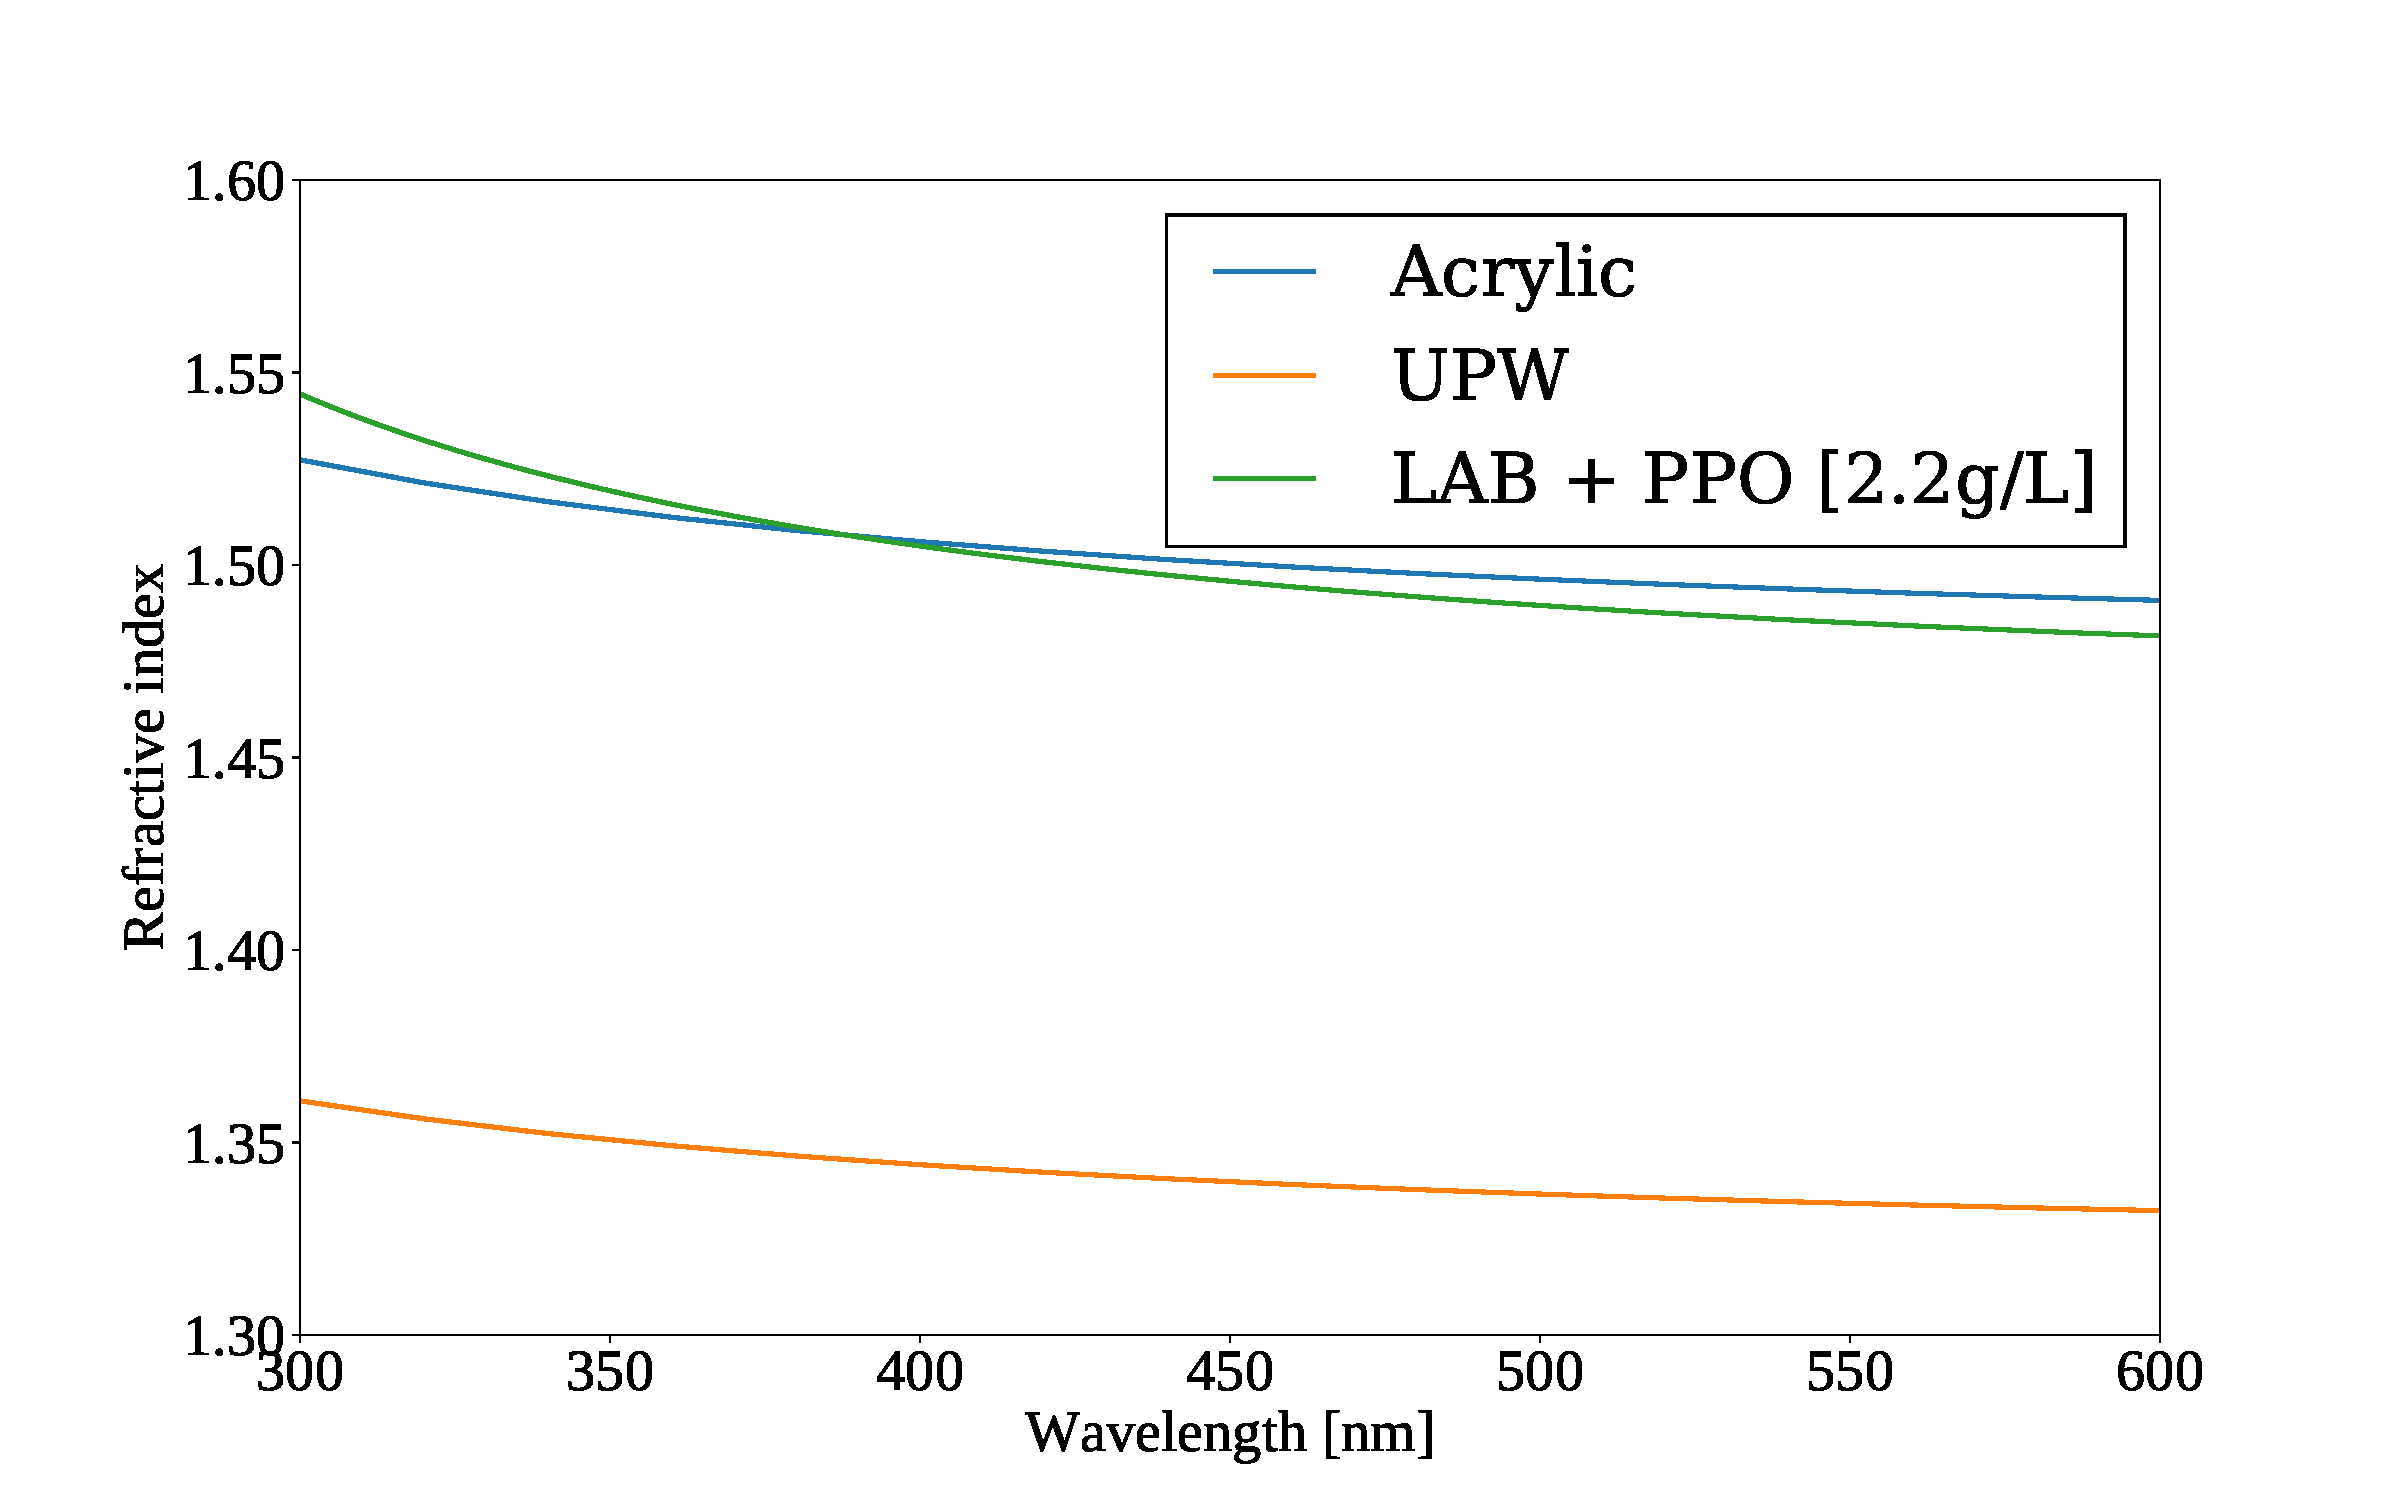
\includegraphics[width=0.95\linewidth]{2_Detector/Figs/refractive_indices_plot.pdf}
        \caption{}
        \label{fig:LE_plot_DayaBay}
    \end{subfigure}
    \begin{subfigure}{0.48\textwidth}
        \centering
        % 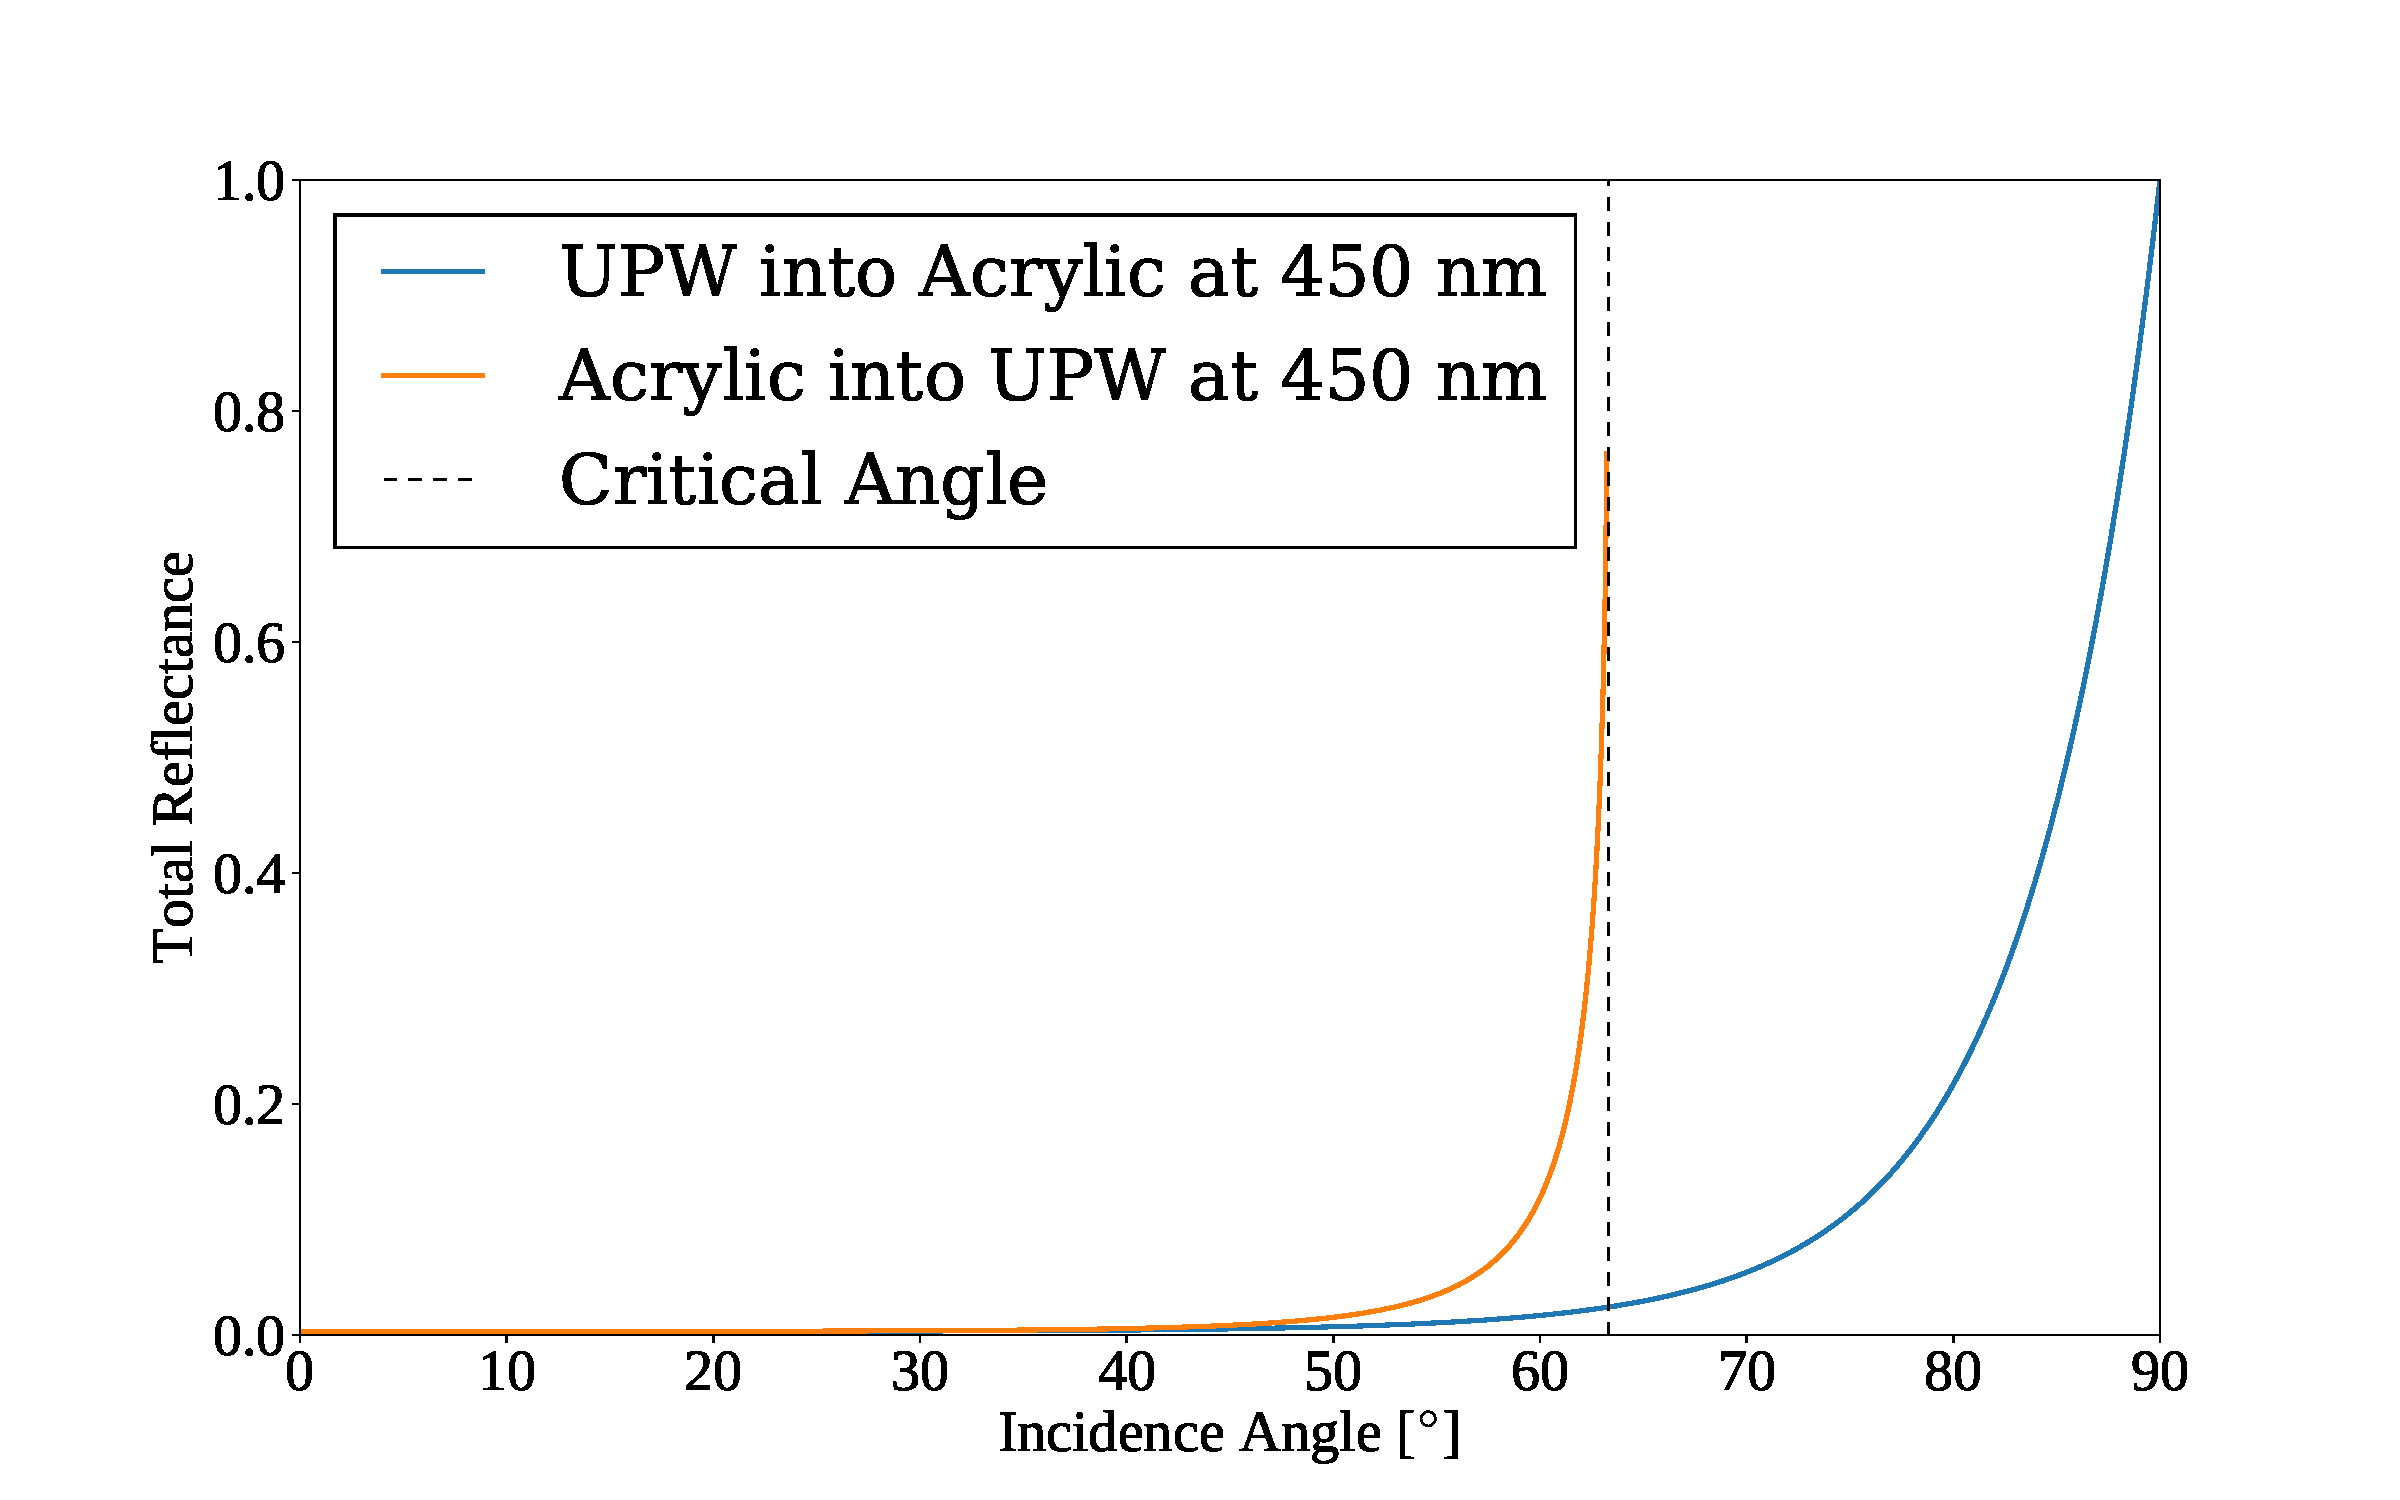
\includegraphics[width=0.95\linewidth]{2_Detector/Figs/reflectance_vs_angle_plot.pdf}
        \caption{}
        \label{fig:LE_plot_4}
    \end{subfigure}
    \caption[]
    {}
    \label{fig:LE_plots}
\end{figure}

\subsubsection{Reactor Anti-neutrinos}
The detection of $\bar{\nu}_{e}$ from nuclear reactors via IBD has been used not just to first detect the existence of neutrinos by Cowan and Reines~\cite{cowanDetectionFreeNeutrino1956,reinesNeutrino1956}, but also to provide evidence for neutrino oscillations. For example, the KamLAND experiment is a large-scale liquid scintillator detector based in Japan in which IBD events can be detected~\cite{}. % cite KamLAND
The expected rate of these events could be derived from the known powers of the various Japanese nuclear reactors, as well as their distances from the experiment. The ratio of the measured rate to expectation as a function of $L_{0}/E$, where $L_{0}$ is the flux-averaged distance to the reactors, is shown in Fig.~\ref{fig:LE_plot_KamLAND_antinu}. The plot shows clear evidence of $\bar{\nu}_{e}$ disappearance, with an oscillatory dependence on $L_{0}/E$.

The Daya Bay, Double Chooz, and RENO experiments are all also liquid scintillator detectors that measured IBD interactions from reactors, but unlike KamLAND they were each placed only $\sim\SI{1}{\km}$ from a nuclear reactor. Each detector observed $\bar{\nu}_{e}$ disappearance over this much shorter length scale, also with a dependence on energy. The results from Daya Bay, as an example, are shown in Fig.~\ref{fig:LE_plot_DayaBay}. Interestingly, the magnitude of the disappearance observed in these `short-baseline' reactor antineutrino experiments is different to those seen in the `long-baseline' KamLAND experiment.

\subsubsection{Accelerator Neutrinos}

{
\color{blue}
\begin{itemize}
    \item Describe status quo ante of massless nature of neutrinos: BEH mechanism as exists cannot allow for neutrinos to have mass as only left-handed neutrinos have been observed.
    \item Furthermore, strong experimental limits on neutrino masses, from e.g. tritium-decay endpoint measurements by the KATRIN experiment and cosmological inferences from the CMB by the Planck satellite.
    \item But --- then neutrino oscillations are observed over a variety of experiments and contexts. Summarise critical bits of evidence:
    \item Electron neutrino disappearance in solar neutrino experiments, including Ray Davis' Homestake experiment, the SAGE/GALLEX experiments, and SNO. For the latter, the comparison of charged-current and neutral-current modes of interaction was clear evidence of neutrino oscillations over other types of process (e.g. neutrino decay).
    \item Include in the above a brief description of Bahcall's Standard Solar Model.
    \item Muon neutrino disappearance in atmospheric and long-baseline accelerator neutrino experiments, such as Super-Kamiokande, T2K, and No$\nu$a.
    \item A few further observations to note are: reactor electron anti-neutrino disappearance from both KamLAND and Daya Bay; tau neutrino appearance at the OPERA experiment; short-baseline neutrino anomaly within LSND and MiniBooNE (with recent contrary evidence from MicroBooNE).
\end{itemize}
[5 pages]
\subsection{The Phenomenology of Neutrino Oscillations}\label{sec:nu_osc_phenom}
\begin{itemize}
    \item Describe the current phenomenological model of 3-flavour neutrino oscillations that can explain all of this evidence: the PMNS mixing matrix.
    \item Describe also the MSW effect, which is critical for explaining solar neutrino oscillations.
    \item Show the formula for solar neutrino oscillations, given this MSW effect in both the Sun and Earth. Note the dependence of solar neutrino oscillations on only the ``solar'' oscillation parameters. This is all particularly useful for the solar analysis chapter.
\end{itemize}

\begin{equation}\label{eq:pee_msw}
    P_{ee}\left(\tan2\theta^{M}_{12}, \sin\theta^{M}_{13}, \Delta m^{2}_{21,M}\right) = BLAH
\end{equation}
[3 pages]
\subsection{The Origins of Neutrino Mass}
\begin{itemize}
    \item Observed neutrino oscillations require at least two neutrino mass states to be non-zero. Given constraints of the current SM, two main ways of adding neutrino masses: a Dirac mass term (i.e. allowing for sterile neutrinos), and a Majorana mass term.
    \item For latter, briefly describe what a Majorana particle is, and how with the Seesaw Mechanism (just the simple Type 1 described in-text) one can not only get neutrino masses but also explain their lightness relative to the other massive SM particles. Note that there exist more elaborate versions of this theory.
    \item Furthermore, with reference to the Sakharov conditions, describe qualitatively how the Seesaw Mechanism also allows for possible leptogenesis/baryogenesis in the early Universe, and hence could explain its matter-antimatter asymmetry.
    \item Describe briefly the nuclear physics behind double-beta decay (i.e. why it can happen at all over just normal beta decay), and then how Majorana neutrinos allow for neutrinoless double beta decay, \onbb{}.
    \item Describe the experimental signature of \onbb{}: a spike of events of observed energy equal to the Q-value of the decay.
    \item Note Schecter-Valle Theorem ensures that any observation of \onbb{} must be the result of neutrinos being Majorana. I.e. the Universe cannot conspire against us and have \onbb{} without Majorana neutrinos.
    \item Very briefly note the current status of the search for \onbb{}, describing the main varieties of experimental setup seen, along with a nice canonical example of such an experiment and their best limit. In particular, the Germanium-crystal detectors such as GERDA, Xenon-TPC detectors like EXO-200, and large-scale liquid scintillators such as KamLAND-Zen.
\end{itemize}
[3 pages]

[CHAPTER TOTAL: 17 pages]
}